\documentclass[25pt,a0paper]{tikzposter}

%% Tikzposter is highly customizable: please see
%% https://bitbucket.org/surmann/tikzposter/downloads/styleguide.pdf

%% Available themes: see also
%% https://bitbucket.org/surmann/tikzposter/downloads/themes.pdf
% usetheme{Default}
% \usetheme{Rays}
% \usetheme{Basic}
% \usetheme{Simple}
% \usetheme{Envelope}
\usetheme{Wave} 
% \usetheme{Board}
% \usetheme{Autumn}
% \usetheme{Desert}
\useblockstyle{Basic} 
%% Further changes to the title etc is possible
% \usetitlestyle{Default}
% \usetitlestyle{Basic}
% \usetitlestyle{Empty}
% \usetitlestyle{Filled}
% \usetitlestyle{Envelope}
% \usetitlestyle{Wave}
% \usetitlestyle{verticalShading}
\usepackage[usenames,dvipsnames]{color}
\usepackage{fontspec}
\usepackage{graphicx}
\usepackage{lipsum}
\setmainfont{FreeSerif}
\setsansfont{FreeSans}
\usepackage{todonotes}
\usepackage[T1]{fontenc}
\usepackage{tgheros}

\newcommand{\TD}[1]{\textcolor{magenta}{\bf [To do] #1}}

\author{\texttt{Marcus Haberland, Deniz Soyuer, Lorenz Zwick,  Lavinia Heisenberg, Prasenjit Saha}}
\title{\parbox{\linewidth}{\centering\texttt{\textbf{Exoplanets around LISA Verification Binaries}}}}
\institute{\texttt{ETH Zurich, University of Zurich}}
%% Optional title graphic
% \titlegraphic{\includegraphics[width=7cm]{IMG_1934}}
%% Uncomment to switch off tikzposter footer
\tikzposterlatexaffectionproofoff

\begin{document}
\maketitle


\block{\centering{\color{white}\texttt{Laser Interferometer Space Antenna as an Exoplanet Detector}}}{
\vspace{-1.cm}
\begin{tikzfigure}
% \hspace{10cm}
\hbox to \hsize{
    \vbox{\hsize=.5\hsize 
    
\begin{itemize}\setlength\itemsep{1.4em}
{\fontfamily{qhv}
    \item \textit{The launch of the \textbf{Laser Interferometer
Space Antenna} \textbf{(LISA)} is currently planned for 2037.
    \item With the first ever detection of \textbf{gravitational waves} (GW), namely GW150914, GW astronomy has \\
    officially become a key part in \textbf{multi-messenger astronomy}.
    \item Recent years have seen the investigation of a \textbf{novel detection method} for exoplanets around GW \\ emitting binary star systems.
    \item This technique$^{[1]}$ is conceptually similar to that of radial  velocity measurements, where \textbf{the orbital \\ motion of an exoplanet induces a detectable Doppler
    shift in the GW frequency of the binary \\system}, rather than its electromagnetic spectrum.
    \item Dozens of galactic binaries have been identified as so called "LISA verification binaries"; \textbf{loud,\\ galactic, ultracompact GW sources with electromagnetic counterparts}.$^{[2]}$
    \item The diagram shows the geometric setup of a compact binary with a circumbinary planet.
    }}
\end{itemize}

    
    } \hss
    \vbox{\hsize=.399\hsize
    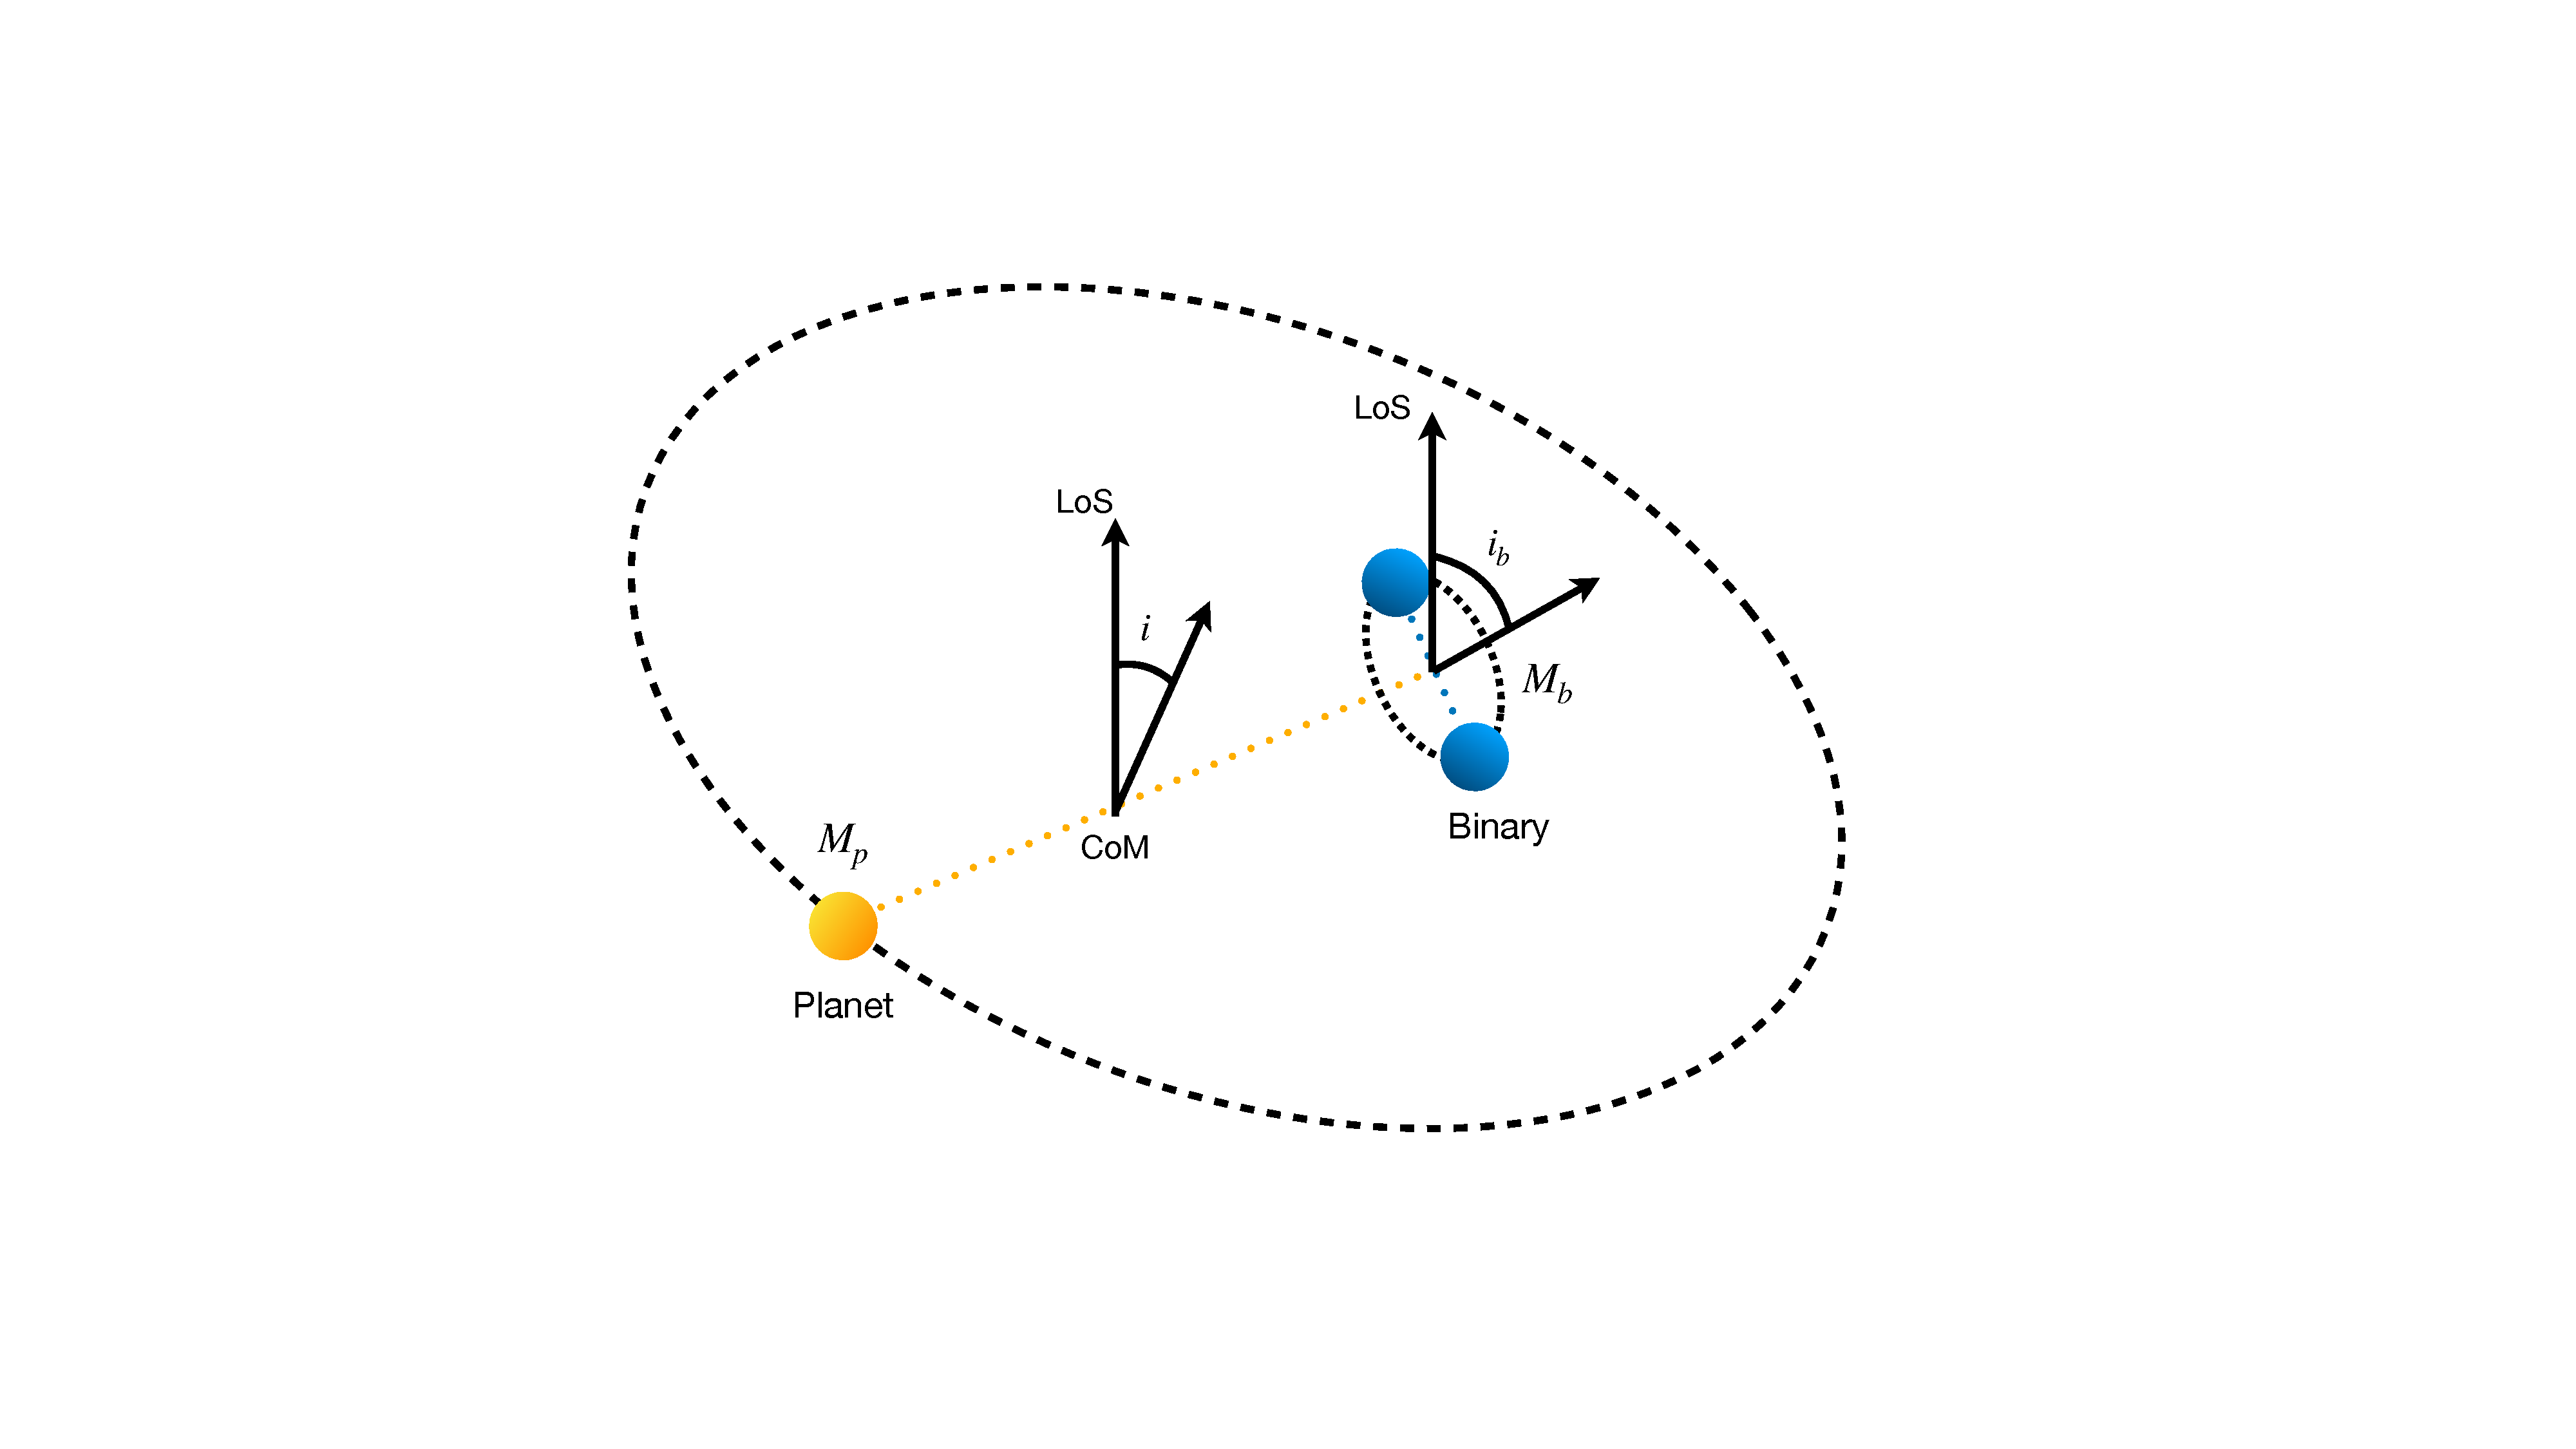
\includegraphics[width = 0.385\columnwidth]{exo_diag.pdf}}}
    %\caption{Some text here}
    \label{fig:my_label}
\end{tikzfigure}
\vspace{1.5cm}
\centering
{\color{purple} 
{\fontfamily{qhv}
    \textit{We investigate whether the \textbf{presence of an exoplanet} could leave a \textbf{detectable imprint} for LISA measurements in the \textbf{GW emission} of verification binaries!}}
}
\vspace{-0.3cm}
}



\block{\centering{\color{white}\texttt{Methods and Analysis}}}{
% \begin{tikzfigure}
% \hspace{10cm}
\hbox to \hsize{%
\vtop{\hsize=.45\hsize\null
      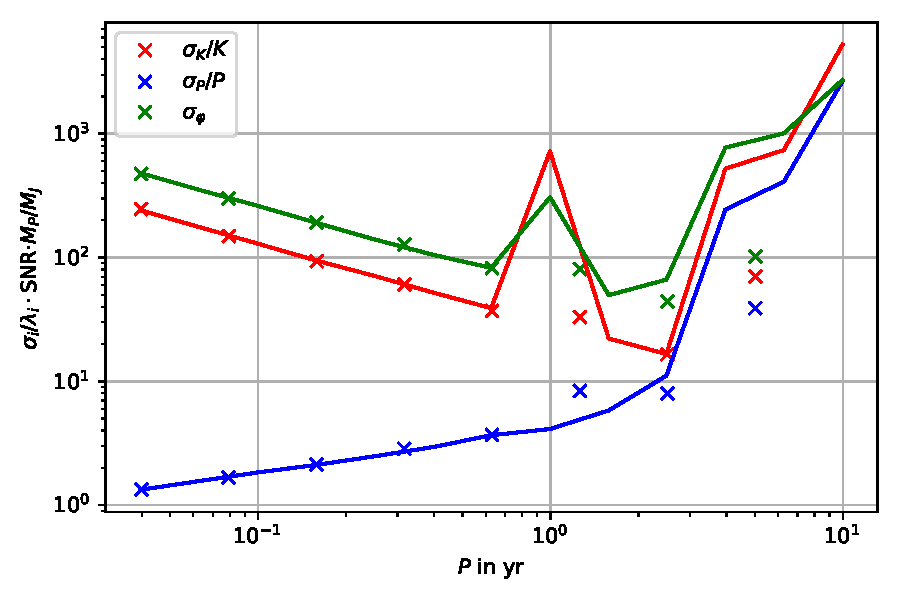
\includegraphics[width=0.9\hsize]{Relative_Uncertainties_l.pdf}}%
\hbox to -.047\hsize{\hfil}%
\vtop{\hsize=.0\hsize \null   
\begin{itemize}\setlength\itemsep{1.em}
\fontfamily{qhv}
    \item  \textit{The \textbf{Fisher information approach} lets us predict the \textbf{recoverable uncertainties of system} \\\textbf{parameters} $\sigma_i$ and correlations $\mathrm{cov}(i,j)$ over the detector lifetime by assuming stationary Gaussian \\noise characterised by a \textbf{noise spectral density} $S_n(f)$ in the limit of \textbf{high} SNR.
    \item  One can calculate the \textbf{Fisher matrix} by numerically performing the integration for a\textbf{ nearly mono-}
    \\\textbf{chromatic signal} by
$\Gamma_{ij} = \frac{2}{S_n(f_0)} \int_0^{T_\mathrm{obs}} \partial_i h(t) \partial_j h(t) \mathrm{d}t$ and then by taking \textbf{the inverse} of the Fisher\\ information to recover
the expected \textbf{covariance matrix} in the parameters $\lambda_i,$ and $\lambda_j$.
\item Panel shows \textbf{relative uncertainties} in the determination of the\textbf{ planet's period} $P$, \textbf{it's initial} \textbf{phase} \\$\varphi_0$ and the parameter $K = \frac{2\pi G}{P}^{1/3} \frac{M_P}{(M_b + M_P)^{2/3}}\sin{i}$ related to the \textbf{minimum mass} for LISA, \textbf{normalized}\\\textbf{ by the SNR} and \textbf{exoplanet mass} (solid lines), \textbf{if we have no prior information about the system.}
\item The \textbf{uncertainties scale as} $\sigma_i \propto \mathrm{SNR}^{-1}$ killing the explicit dependence on the strain sensitivity $S_n(f)$.
\item LISA is unable to detect Jupiter-like circumbinary planets with no prior information about the source \\ position, \textbf{which is not the case for verification binaries} (see next panel).
% \item The resulting relative uncertainties for an circumbinary planet are recovered by dividing by \\the binary's $S/N$ and the exoplanet's mass $M_P$.
}\end{itemize}
}%
}


}


\block{\centering{\color{white}\texttt{Challenges and Inclusion of Doppler Tracking}}}{
% \vspace{-0.5cm}
\begin{tikzfigure}
% \hspace{10cm}
\hbox to \hsize{
    \vbox{\hsize=.5\hsize 

\fontfamily{qhv}
\hspace{-32cm}\textbf{Challenges:}
\begin{itemize}\setlength\itemsep{0.5em}
\fontfamily{qhv}
    \item \textit{One needs high signal-to-noise ratios SNR $\gg$ 1 of the binary in order to observe 
    the signal of an \\exoplanet, strongly
reducing the number of candidate systems. 
\item  As with classical
RV techniques, this method is strongly biased to favor massive
planets with \\orbital periods P comparable to the nominal mission
life-time. 
\item As space-borne missions
orbit the sun next to Earth, planets with periods comparable to
a multiple \\ of one year can’t be resolved because of a high correlation with the detectors orbit. For verification \\binaries, this degeneracy vanishes.}
\end{itemize}
\vspace{1cm}
\fontfamily{qhv}
\hspace{-12.3cm}\textbf{Doppler Tracking Missions to Uranus and Neptune:}
\begin{itemize}\setlength\itemsep{0.5em}
{\fontfamily{qhv}
    \item \textit{Recent years have seen numerous publications underlining the importance of a \textbf{space mission} to \\the \textbf{ice giants} in the upcoming decade that involve a 10 yr cruise time. The cruise time can be \\ \textbf{utilized to search for GWs} by observing the \textbf{Doppler shift} caused by them in their \textbf{radio link}.$^{[3]}$ 
    \item Panel shows the uncertainties in determination of $P$, $\varphi_0$, $K$ for random sources by LISA (solid lines) \\ an ice giant Doppler tracking mission  \textbf{for verification binaries} (dashed), and with LISA (triangles). \\Naturally, the SNR will be \textbf{much lower} for the Doppler tracking mission than for LISA.
    }}
\end{itemize}

    } \hss
    \vbox{\hsize=.41\hsize
    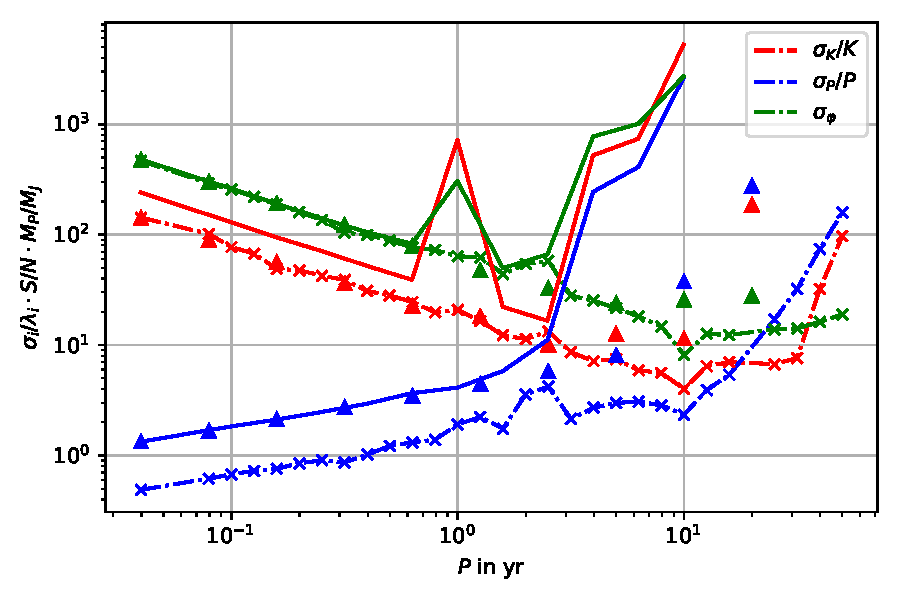
\includegraphics[width = 0.384\columnwidth]{Tamanini_comp.pdf}}}
    %\caption{Some text here}
    \label{fig:my_label}
\end{tikzfigure}
\centering
{\color{purple} 
{\fontfamily{qhv}
    \textit{Thus, \textbf{prospective ice giant missions} with sufficient Doppler tracking capabilities can help constrain exoplanet parameters \textbf{along with LISA}, around verification binaries.}}
} 

}

\block{\centering{\color{white}\texttt{References }}}{
\small

$^{[1]}$ \texttt{\textbf{Tamanini, N. & Danielski, C. 2019} The gravitational-wave detection of exoplanets orbiting white dwarf binaries using LISA, \textit{Nature Astronomy}
 ~~~~~~~~~~~~~~~~~~~~~~~~~~~~~~~~~~~Email:\! marcush@student.ethz.ch,}


$^{[2]}$ \texttt{\textbf{Kupfer, T et al. 2018:} LISA verification binaries with updated distances from Gaia Data Release 2, \textit{MNRAS}~~~~~~~~~~~~~~~~~~~~~~~~~~~~~~~~~~~~~~~~~~~~~~~~~~~~~~~~~~~~~~~~~~~~~~~~~~~~soyuerd@ics.uzh.ch,}


$^{[3]}$ \texttt{\textbf{Soyuer D. et al. 2021: }Searching for gravitational waves via Doppler tracking by future missions to Uranus and Neptune, \textit{MNRAS}~~~~~~~~~~~~~~~~~~~~~~~~~~~~~~~~~~~~~~~~~~~~~~~~~~~~~~~zwicklo@ics.uzh.ch}



}
\end{document}
